\part{Análisis Matemático}
\chapter{Preámbulos para análisis}
\minitoc

\newpage
\section{Topología sobre $\mathbb{R}$}
La topología ocupa un lugar muy destacado cuando se trata del análisis matemático ya que es la rama que estudia que ocurre con ciertas propiedades de proximidad cuando a un conjunto le aplicas lo que hemos llamado funciones continuas en anteriores cursos. 

\begin{defi}
Una \textbf{topología}, $\tau$, sobre el conjunto $A$  es una familia de subconjuntos de  finita o no que cumple las siguientes características:
\begin{itemize}
\item $A$ y $\emptyset$ pertenecen a $\tau$.
\item Dado $\lbrace A_i \rbrace_{i\in I}$ una familia arbitraria (puede ser finita o no) de elementos de $\tau$ entonces $\cup_{i\in I} A_i$ también pertenece a la topología.
\item Dado $\lbrace A_i \rbrace_{i=0}^{i=k}$ una familia finita de elementos de la topología entonces $\cap_{i=0}^{i=k} A_i$ es también un elemento de la topología.
\end{itemize}

A esta forma de definir una topología lo llamamos definir una topología por \emph{abiertos}, ya que a los elementos de la topología definida así se les llama conjuntos abiertos. 
\end{defi}
\begin{ejercicio}
Comprobar que $\mathbb{R}$ con los intervalos abiertos es una topología. 
\end{ejercicio}

\begin{defi}
Diremos que un conjunto es \textbf{cerrado} cuando su complementario sea abierto. 
\end{defi}

\paragraph*{Aclaración: } Un conjunto puede no ser ni abierto ni cerrado y puede ser los dos a la vez, como por ejemplo el $\emptyset$ ya que su contrario que sería el total es abierto, pero como está en la topología $\tau$, entonces es abierto. Ambas cosas no son contradictorias. 

Ahora bien, supongamos que ya tenemos estas cualidades de espacio topológico, ahora vamos a definir lo que es un entorno abierto de un punto a. 
\begin{defi}
Un entorno no es más que la vecindad de un punto \emph{(Los puntos cercanos a él)}, y diremos que un entorno $E$ es abierto si $\forall x \in E $ existe un abierto que está contenido en el entorno. 

\end{defi}

Ahora nos falta definir una medida sobre $\mathbb{R}$ que nos permita decir de manera clara y concisa lo que está y lo que no está en las vecindades del punto. La medida más habitual sobre $\mathbb{R}$ es el valor absoluto. 


\begin{defi}
Una medida es una aplicación 
$$
\begin{array}{rccl}
||  \colon & \mathbb{R} \times \mathbb{R} & \longrightarrow & \mathbb{R}\\
&(x,y) & \longmapsto & dist(x,y)
\end{array}
$$
\noindent
Que cumple las siguientes propiedades:
\begin{itemize}
\item $\forall x \in \mathbb{R} $ se cumple que $dist(x,x)=0$
\item $\forall x,y\in \mathbb{R}$ se cumple que $dist(x,y)=dist(y,x)$ 
\item $\forall x,y,z \in \mathbb{R}$ se cumple que $dist(x,z)\leq dist(x,y)+dist(y,z)$ Es decir, el camino más corto es el camino directo entre dos puntos.
\end{itemize}

\end{defi}

\begin{ejercicio}
Probar que el valor absoluto es una medida sobre los números reales. 
\end{ejercicio}

Ahora, vamos a definir la principal definición para la que usamos la topología. Las funciones continuas. 

\begin{defi}
Una aplicación
$$
\begin{array}{rccl}
f  \colon & X & \longrightarrow & Y\\

\end{array}
$$
Diremos que es continua si $\forall E$ abierto de $B$ entonces se cumple que $f^{-1}(B)$ es oto conjunto abierto. 
\end{defi}

Esta definición nos quiere decir que este tipo de funciones lo que hace es mandar puntos que están cerca a puntos que siguen cerca por así decirlo,ya que un entorno de f(a) viene de un entorno de a.


Continuará...


\chapter{Cálculo de Límites}
\minitoc

\newpage

\section{Preámbulo sobre las sucesiones reales}
\begin{defi}
Definimos una sucesión de números reales $\lbrace a_k \rbrace$ como una aplicación de la forma: 
$$
\begin{array}{rccl}
\lbrace a_k \rbrace  \colon & \mathbb{N} & \longrightarrow & \mathbb{R}\\
& k & \longmapsto & a_k
\end{array}
$$
\end{defi}
\noindent
Tenemos que tener claros unos cuantos conceptos sobre sucesiones antes de ponernos a definir lo que es una función o sucesión convergente y que es eso de convergente. 

\begin{defi}
Se dice que una sucesión $\lbrace a_n \rbrace$ es convergente en $\mathbb{R}$, o que es convergente a $l\in \mathbb{R}$ o que su límite es $l$ cuando si $\forall \varepsilon \geq 0$ y $\varepsilon \in \mathbb{R}$ $\exists n_0\in \mathbb{N}$ de manera que cuando $n\leq n_0\Leftarrow |l-a_n|\leq \varepsilon$
\end{defi}

\paragraph*{\textit{Aclaración:}} Una sucesión que sea convergente tiene un único límite.\\[2ex]
\noindent
Esta definición lo que nos dice es que cogiendo un $\varepsilon$ arbitrariamente pequeño se puede encontrar un $n_0 \in \mathbb{N}$ de manera que la distancia entre el límite y un término posterior de $\lbrace a_n \rbrace$ a $a_{n_0}$ es menor que ese $\varepsilon$\\

\noindent
Podemos entonces extender esta definición a una aplicación del tipo
\begin{equation*}
\begin{array}{rccl}
f \colon & \mathbb{R} & \longrightarrow & \mathbb{R}\\

\end{array}
\end{equation*}

Entonces dejemos definido esta extensión a lo continuo 
\section{Definición}

\begin{defi}
Una función es convergente a $l$ cuando $x\to a$ $\forall \varepsilon \in \mathbb{R}$ entonces $\exists \delta \geq 0 $ de manera que $|x-a|\leq \delta \Rightarrow |f(x)-f(a)|\leq 0$
\end{defi}

Podemos definir de esta manera el límite ya que hemos definido la estructura de espacio métrico de $\mathbb{R}$ ya que como demostramos anteriormente esta aplicación es una distancia. 

\begin{ejercicio}
Probar que la función $f(x)=x^2+x+1$ tiende a 1 en el punto $x=0$
\end{ejercicio}
\begin{proof}
Tomemos un $\varepsilon < 0$ entonces tomando como $\delta < min\lbrace 1, \dfrac{\varepsilon}{2}\rbrace\Rightarrow \delta <1 \Rightarrow \delta^2 <\delta$ por tanto, tenemos que $|x|<\delta$  

\begin{equation*}
|f(x)-1|=|x^2+x|\leq |x^2|+|x|< \delta^2+\delta<2\delta < \varepsilon
\end{equation*}
\end{proof}

\section{Propiedades de los límites}

\noindent
Una función puede tener distintos límites dependiendo de que topología esté definida sobre el conjunto a estudiar pero hay que recordar que una vez fijada la topología, este es único.
\noindent


Ahora vamos a ver y a comprender ciertas propiedades que nos ayudarán en el cálculo efectivo de límites\\[2ex]

\begin{proposicion}
Sean $f, g$ dos funciones cuyos límites $\lim_{x\to a} f$ $\lim_{x\to a} f$ existen entonces 
\begin{itemize}
\item $\displaystyle\lim_{x\to a}(f+g)(x)=\lim_{x\to a}f(x)+ \lim_{x\to a} g(x)$
\item $\displaystyle\lim_{x\to a} (f\cdot g)(x)=\lim_{x\to a}f(x)\cdot \lim_{x\to a}g(x)$
\item Sea $\lambda \in \mathbb{R}$ entonces $\displaystyle\lim_{x\to a}\lambda f(x)=\lambda \lim_{x\to a} f(x)$
\item Si se cumple que $\displaystyle\lim_{x\to a} g(x)\neq 0$ entonces $\displaystyle\lim_{x\to a} \dfrac{1}{g(x)}=\dfrac{1}{\lim_{x\to a} g(x)}$
\end{itemize}
\end{proposicion}
\section{Cálculo efectivo de límites}

Sea 

\section{Indeterminaciones}



%%Capítulo 7



\chapter{Las funciones sobre $\mathbb{R}$}
\minitoc

\newpage

\section{Definiciones previas}

\begin{defi}
Una función $f(x)$ es continua en un punto a cuando $\displaystyle \lim_{x\to a} f(x)=f(a)$. Es otra forma de definir la continuidad y es equivalente a la definición que se puede dar de una aplicación continua que dábamos en el apartado de topología. 
\end{defi}

\begin{defi}
Diremos que una función es continua si lo es en todos sus puntos. 
\end{defi}

\paragraph*{Propiedades}
Se cumplen las siguientes propiedades asociadas a las funciones continuas:
\begin{itemize}
\item Dadas $f$ y $g$ dos funciones continuas entonces tendremos que $f+g$ también es una función
\item Dada $f$ una función continua y $k\in \mathbb{R}$ entonces tenemos que $k\cdot f$ es una función continua también 
\item Dadas dos funciones $f, g$ continuas tenemos que $f\cdot g$ también es continua
\item La composición de funciones continuas $f,g$ también es una función  continua. 
\end{itemize}

\begin{ejercicio}
Demostrar mediante las propiedades de los límites de linealidad y de conservación del producto.
\end{ejercicio}

\begin{ejercicio}
Comprueba si las siguientes funciones son continuas en $x=2$
\begin{equation*}
\begin{array}{rrrr}
a) f(x)=\dfrac{1}{x-2}& b)f(x)=\dfrac{3x-5}{x^2-4}& c)f(x)=\dfrac{x^2}{x^2+1}& d)f(x)=3x^2-\dfrac{2}{x}\\
\end{array}
\end{equation*}

Comprobar que una función es continua en un punto $x=a$ es únicamente comprobar que el $\displaystyle lim_{x\to a} f(x)=f(a)$ por tanto hay que tener en cuenta cuando no existe un límite



\end{ejercicio}



%%Capítulo 8


\chapter{Derivabilidad sobre $\mathbb{R}$}

\minitoc

\newpage


\section{Concepto de la derivada}
Para empezar, tenemos que refrescar un concepto de geometría análitica, \emph{la pendiente de una recta}
\begin{defi}
La pendiente de una recta en $\mathbb{R}^2$ \emph{(El plano real)} se define como la cantidad de unidades que avanza la $y$ por cada unidad que avanza la $x$. Es decir, definiendo el incremento de y como $y_1-y_0=\Delta y$ donde $y_1$ es la coordenada y del punto final y $y_0$ lo mismo pero del punto inicial. definimos de manera igual el $\Delta x$. Entonces definimos de manera matemática la fórmula de la pendiente como :
\end{defi}
\begin{equation*}
m=\dfrac{\Delta y}{\Delta x}
\end{equation*}

\noindent
Ahora bien, sea $f(x)$ una función de manera que $f:\mathbb{R}\longrightarrow \mathbb{R}$ de la cual queremos obtener la recta secante que pasa por unos determinados puntos $p_1=(x_1,y_1),p_2=(x_2,y_2)$. Entonces tendremos la siguiente gráfica:\\
\noindent
Tendremos entonces que la fórmula de la recta secante a la función que pasa por esos dos puntos $p_1,p_2$ es la siguiente:
\begin{equation*}
(y-f(x_1))=\dfrac{\Delta f(x)}{\Delta x}(x-x_1)
\end{equation*}
\begin{defi}
A la pendiente de la recta secante a la función $f(x)$ en los puntos $x_1,x_2$ se le conoce como \textbf{\emph{Tasa de Variación Media}}
\end{defi}

\noindent
Supongamos ahora que escribimos $x_1=x$ y $x_2=x+h$ donde $h\in \mathbb{R}$ entonces la ecuación anterior queda como:
\begin{equation*}
(y-f(x_1))=\dfrac{f(x_1+h)-f(x_1)}{h}(x-x_1)
\end{equation*}

\noindent
Si después de esto, si hacemos que la $h\to 0$ obtendremos la recta tangente de manera que la pendiente  $\displaystyle \lim_{h\rightarrow 0}\dfrac{f(x+h)-f(x)}{h}$.

\noindent
Es ese límite lo que definimos como \emph{Derivada de una función}.
\begin{defi}
Llamaremos derivada de $f(x)$ en el punto $a$ al límite
\begin{equation*}
\lim_{h\to 0}\dfrac{f(a+h)-f(a)}{h}
\end{equation*}

\end{defi}
\newpage
\section{Derivabilidad de una función}
\begin{defi}
Diremos que una función es derivable en $a$ si existe el límite $\displaystyle \lim_{h\rightarrow 0}\dfrac{f(x+h)-f(x)}{h}$.
\end{defi}
\begin{defi}
Diremos que una función es derivable si lo es en todos los puntos del dominio.
\end{defi}
\subsection{Estudio de la derivabilidad de una función}

\newpage
\section{Tabla de derivadas}
\subsection*{Propiedades de la derivada}
Para empezar hay que tener en cuenta estas derivadas de operaciones de funciones básicas, sumar y restar, producto y división, producto por un escalar y composición\\[2ex]

\begin{tabular}{l l}
$(f(x)+g(x))'=f'(x)+g'(x)$ & $(f(x)-g(x))'=f'(x)-g'(x)$\\
$(f(x)\cdot g(x))'=f'(x)g(x)+g'(x)f(x)$& $\left(\dfrac{f(x)}{g(x)}\right)'=\dfrac{f'(x)g(x)-g'(x)f(x)}{g^2(x)}$\\
$(\lambda\cdot f(x))'=\lambda f'(x)$ $\forall \lambda \in \mathbb{R}$& \\
Regla de la cadena: $(f\circ g (x))'=f'(g(x))\cdot g'(x) $&\\
 & \\
\end{tabular}

\noindent
Estas son las propiedades básicas de todas las derivadas, la mayoría se demuestran con la definición de la derivada como un límite. 
\noindent
Ahora veamos la tabla de la fórmulas de las derivadas habituales 
\begin{center}
\begin{tabular}{|l|l|l|}
\hline
Nombre de la función& Derivada & Composición\\[2ex]
\hline
Potencial &$(x^n)'=n x^{n-1}$&$(f(x)^n)=n f(x)^{n-1}\cdot f'(x)$\\[2ex]
\hline
Exponencial en base e &$(e^x)'=e^x$&$(e^{f(x)})=e^{f(x)}\cdot f'(x)$\\[2ex]
\hline
Exponencial en base a &$(a^x)'=a^x\cdot ln(a)$&$(a^{f(x)})=a^{f(x)}\cdot f'(x)\cdot ln(a)$\\[2ex]
\hline
Logaritmo en base a &$(log_a(x))'=\dfrac{1}{x\cdot ln(a)}$&$(log_a(f(x)))'=\dfrac{f'(x)}{ln(a)\cdot f(x)}$\\[2ex]
\hline
Logaritmo neperiano &$(ln(x))'=\dfrac{1}{x}$&$(ln(f(x)))'=\dfrac{f'(x)}{f(x)}$\\[2ex]
\hline
Coseno &$(cos(x))'=sen(x)$&$(f(x)^n)=n f(x)^{n-1}\cdot f'(x)$\\[2ex]
\hline
Seno &$(sen(x))'=-cos(x)$&$(f(x)^n)=n f(x)^{n-1}\cdot f'(x)$\\[2ex]
\hline
Tangente&$(tg(x))'=1+tg^2(x)$&$(f(x)^n)=n f(x)^{n-1}\cdot f'(x)$\\[2ex]
\hline
Arcoseno &$(arcsen(x))'=n x^{n-1}$&$(f(x)^n)=n f(x)^{n-1}\cdot f'(x)$\\[2ex]
\hline
Arcocoseno &$(x^n)'=n x^{n-1}$&$(f(x)^n)=n f(x)^{n-1}\cdot f'(x)$\\[2ex]
\hline
Arcotangente &$(x^n)'=n x^{n-1}$&$(f(x)^n)=n f(x)^{n-1}\cdot f'(x)$\\[2ex]
\hline

\end{tabular}
\end{center}

\newpage
\section{Algunas demostraciones de fórmulas de derivadas}






%%Capítulo 9



\chapter{Aplicaciones de la derivada}
\minitoc

\newpage
\section{Cálculo de mínimos y máximos}
\section{Cálculo de la curvatura de las funciones}
\section{Optimización de funciones}



%%Capítulo 10



\chapter{Representación de funciones}
\minitoc

\newpage
\section{Dominio}
Recordemos lo que era el dominio de una función de manera precisa
\begin{defi}
El dominio de una función o aplicación $f: X\longrightarrow Y$ es el subconjunto de puntos $x \in X$ para el cual existe $f(x)$. 
\end{defi}
\noindent
Para que lo entendamos de nuevo la función $f$ en el caso que nos ocupa es algo a lo que le entran números, la función hace una operación, \emph{(En el caso de $2x$ sería que lo multiplica por dos)} y te devuelve ese valor operado. 
\noindent
El dominio son los números que la función puede operar sin  romperse, es decir, sin hacer cosas raras que no se pueden hacer en los números reales como por ejemplo:
\begin{itemize}
\item Dividir entre 0: Por tanto si tenemos una fracción habrá que comprobar cuando el denominador se hace 0. (Plantear la ecuación)
\item Hacer la raíz de un número negativo: Para poder hacerlo tendríamos que extender nuestro campo a $\mathbb{C}$ lo cual ahora mismo se nos escapa de nuestro alcance. Se plantea la inecuación
\item Hacer el logaritmo de un número negativo 
\end{itemize}

\subsection*{Dominios de las funciones elementales}
\noindent
Ahora vamos a ir desmenuzando los tipos de funciones que conocemos y analizando su dominio:
\begin{itemize}
\item \textbf{Funciones Polinómicas} Son las funciones del tipo $a_n\cdot x^n+\ldots+ a_o$ en este caso, su dominio es todo $\mathbb{R}$.
\item \textbf{Funciones Racionales} Son las funciones del tipo $\displaystyle \dfrac{a_n\cdot x^n+\ldots+ a_0}{b_m\cdot x^m+\ldots+ b_0}$ en este caso, su dominio es todo $\mathbb{R}$, salvo los puntos en los que se anule el denominador, por o tanto hay que resolver la ecuación $b_m\cdot x^m+\ldots+ b_0=0$.
\item \textbf{Funciones Irracionales} Son las de tipo $f(x)=\sqrt[n]{g(x)}$ tenemos que el dominio de $f(x)$ es:
\begin{itemize}
\item El mismo que $g(x)$ si n es \emph{impar}
\item Si n es par el dominio de $f(x)$ son los x que cumplen que  $g(x)\geq 0$. 
\end{itemize}
\item \textbf{Funciones Exponenciales}
Son de la forma $f(x)=a^{g(x)}$ con $a>0$ y $a\neq 1$, su dominio es $\mathbb{R}$.
\item \textbf{Funciones Logarítmicas}
Son de la forma $f(x)=log_a g(x)$ $a>0$ y  su dominio son los $x$ tales que $g(x)>0$.
\item \textbf{Funciones Trigonométricas Circulares} 
Tanto $f(x)=cos(x)$ como $f(x)=sen(x)$ su dominio es $\mathbb{R}$ y de aquí se pueden considerar el resto de funciones trigonométricas. 
\end{itemize}
\section{Simetría y periodicidad}
\noindent
La simetría de una función se define de la siguiente manera:

\begin{defi}
Una función $f:A \longrightarrow \mathbb{R}$ es par si $\forall x \in A$ se cumple que $f(-x)=f(x)$. Es decir, es simétrica respecto del eje de coordenadas $OY$
\end{defi}

\begin{defi}
Una función $f:A \longrightarrow \mathbb{R}$ es impar si $\forall x \in A$ se cumple que $f(-x)=f(x)$. Es decir, es simétrica respecto del origen de coordenadas 
\end{defi}
\begin{figure}[H]
\graphicspath{{imagenes_analisis/}}
\subfloat[Función impar]{
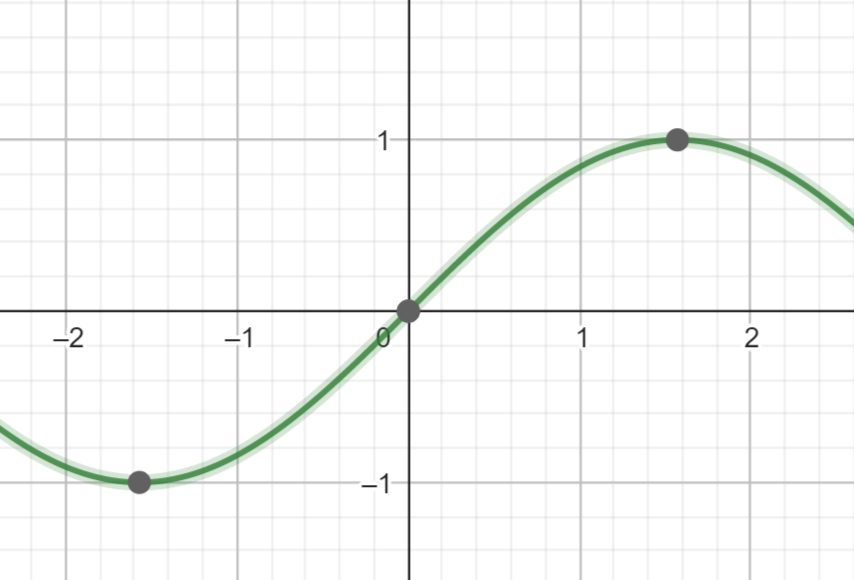
\includegraphics[scale=1.25]{representacion1.png}}
\subfloat[Función par]{

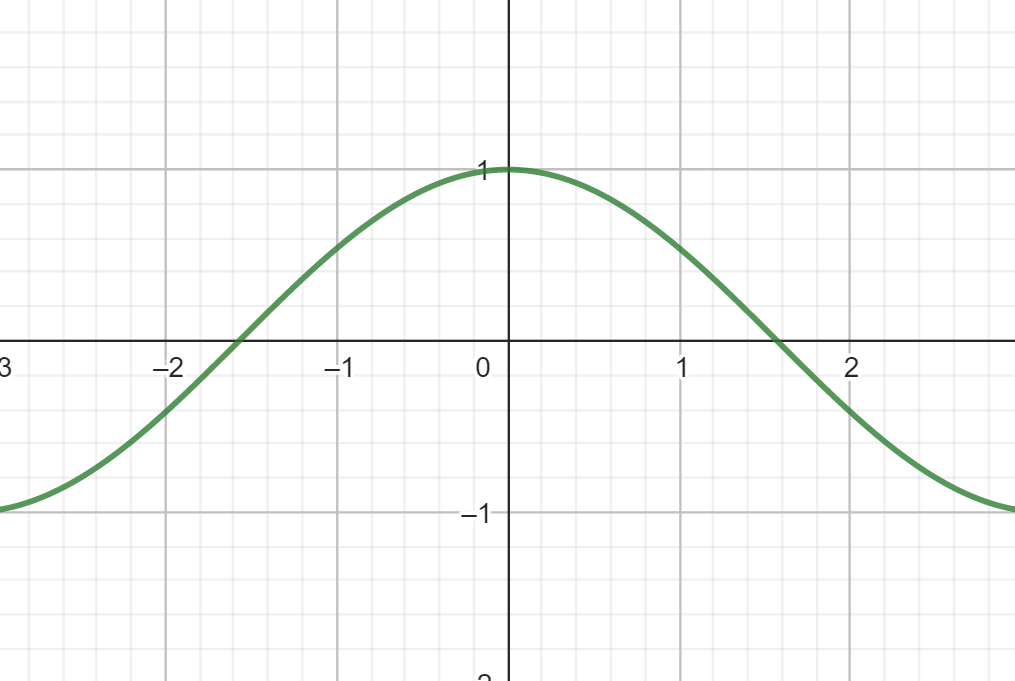
\includegraphics[scale=1.25]{representacion2.png}}

\end{figure}
\noindent
Estas cualidades lo que nos permiten es reducir el tamaño del conjunto de puntos a estudiar, en el caso de la simetría nos permite reducir a la parte positiva de los reales y la periodicidad a un solo periodo. 
\newpage


\section{Continuidad}

La continuidad de una función es una propiedad que se estudia dentro del dominio de una función y aunque no tiene sentido estudiar si se da en puntos que no son del dominio de la función solemos comprobar que pasa en las inmediaciones de los puntos que no pertenecen al dominio, manteniéndonos en el dominio. Es decir, si tengo un dominio que es $\mathbb{R}-\lbrace 0 \rbrace$ haremos el límite de la función cuando $x\to 0 $ para saber que tenemos en las inmediaciones del punto. Tenemos dos casos: 
\begin{itemize}
\item Que la función sea a trozos con ramas continuas a ambos lados del punto que las une
\begin{ejemplo}
%%Mirar como se hacían las ecuaciones diferenciales elípticas en el documento de Calc.Cient
\end{ejemplo}
\item Que la función tenga un punto singular 
\begin{ejemplo}
\end{ejemplo}
\end{itemize}
\newpage
\section{Corte con los ejes}
Los cortes con los ejes son importantes por que nos dan una referencia de donde está situada la gráfica de la curva. 
\begin{itemize}
\item Cortes con el eje X. 
\item Cortes con el eje Y.
\end{itemize}
\section{Asíntotas}
\subsection*{Asíntotas Verticales}
\subsection*{Asíntotas Horizontales}
\subsection*{Asíntotas Oblicuas}
\section{Monotonía}
\section{Curvatura}

\section{Análisis de cada tipo de función elemental}
\subsection*{Polinómicas}
\subsubsection*{Dominio}
\noindent
Las funciones polinómicas tienen como dominio todo $\mathbb{R}$.
\subsection*{Simetría}
\noindent
Solo las funciones que cumplen $P(x)=\sum a_n\cdot x^{2n}$ con $n\neq 0$ son pares  
\subsection*{Continuidad}
\noindent
Los polinomios son funciones continuas en todo $\mathbb{R}$
\subsection*{Asíntotas}
Los polinomios no tienen asíntotas verticales, horizontales ni oblicuas.
\subsection*{Monotonía y curvatura}
No es más que derivar funciones polinómicas. 
\newpage
\begin{ejemplo}
La función $f(x)=x^3+x^2-x-1$ tiene la siguiente función.
En detalle podemos ver que efectivamente el dominio es todo $\mathbb{R}$, no es simétrica, es continua, no tiene asintotas 
\end{ejemplo}
\begin{center}
\begin{figure}[H]
\centering
\graphicspath{{imagenes_analisis/representacion}}
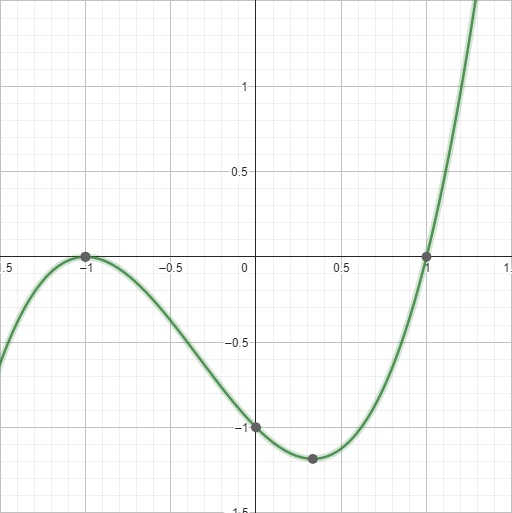
\includegraphics[scale=0.4]{funciones1.png}
\end{figure}
\end{center}





%%Capítulo 11



\chapter{Integración sobre $\mathbb{R}$}
\minitoc

\newpage

\section{Conceptos principales}
\noindent
\textbf{¿Qué demonios es una integral?}\\[1ex]
La integral es una suma, una suma infinita, normalmente se define como el área de bajo la gráfica que forma la curva con el eje de las x's.\\[2ex]
\noindent
Sea una función $f\colon [a,b] \longrightarrow \mathbb{R}^+$ (por ahora vamos a considerar que es únicamente positiva, es decir, solo puede tomar valores positivos). 
\begin{figure}[H]
\begin{center}
\graphicspath{{imagenes_analisis/}}
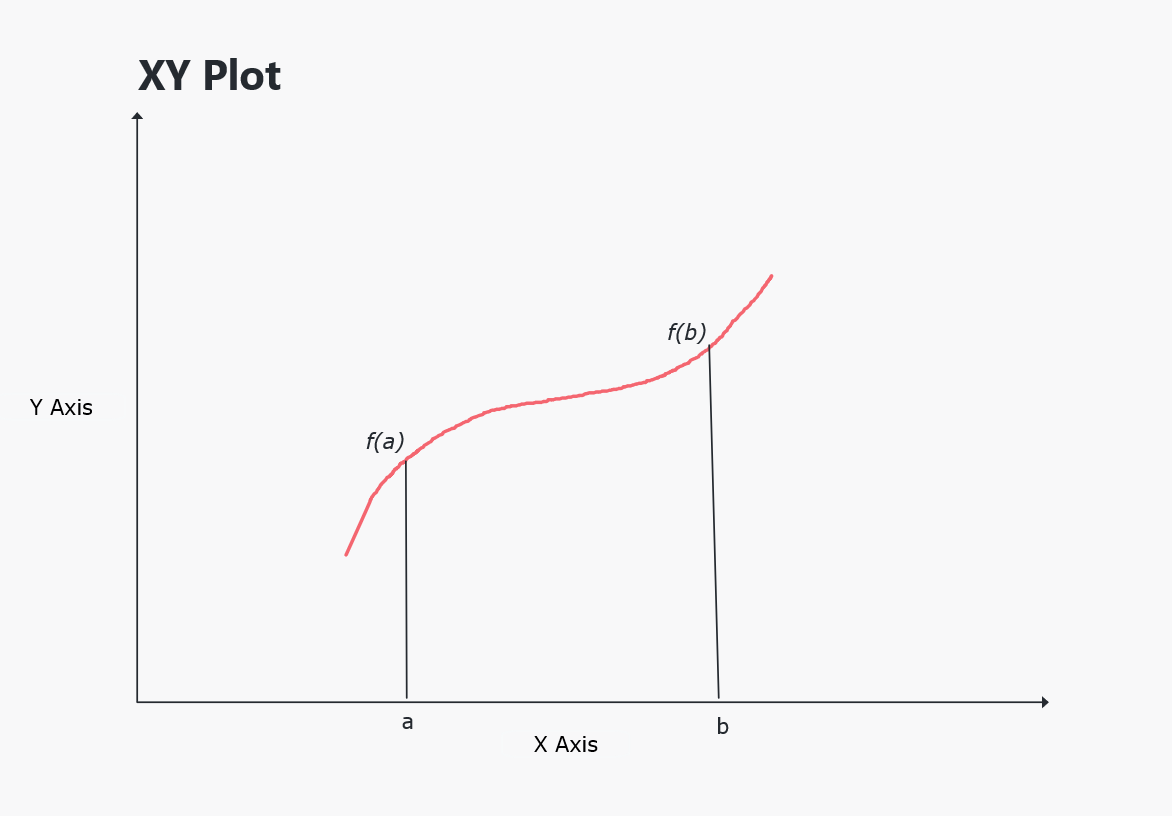
\includegraphics[scale=0.25]{integrales1.png}
\label{Función $f(x)$}
\end{center}
\end{figure}

Entonces podemos hacer una primera aproximación del área por rectángulos . En principio, tenemos un rectángulo que cogiendo el mínimo de la función nos queda como se muestra en la imagen:

\begin{figure}[H]
\centering
\graphicspath{{imagenes_analisis/}}
\subfloat[Área la suma inferior]{

    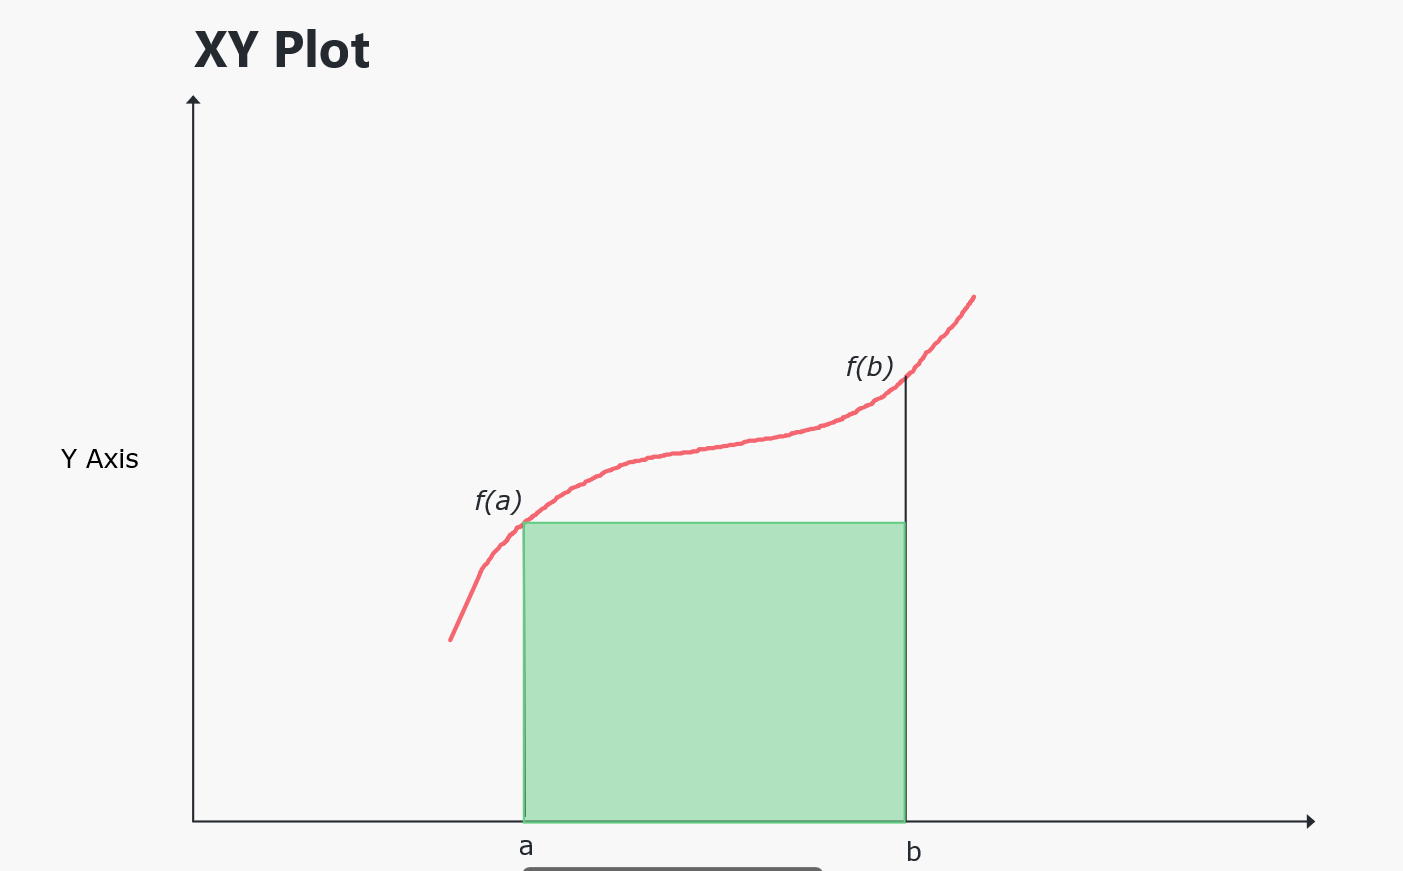
\includegraphics[scale=0.15]{Integrales2.png}}
\subfloat[Área la suma superior]{

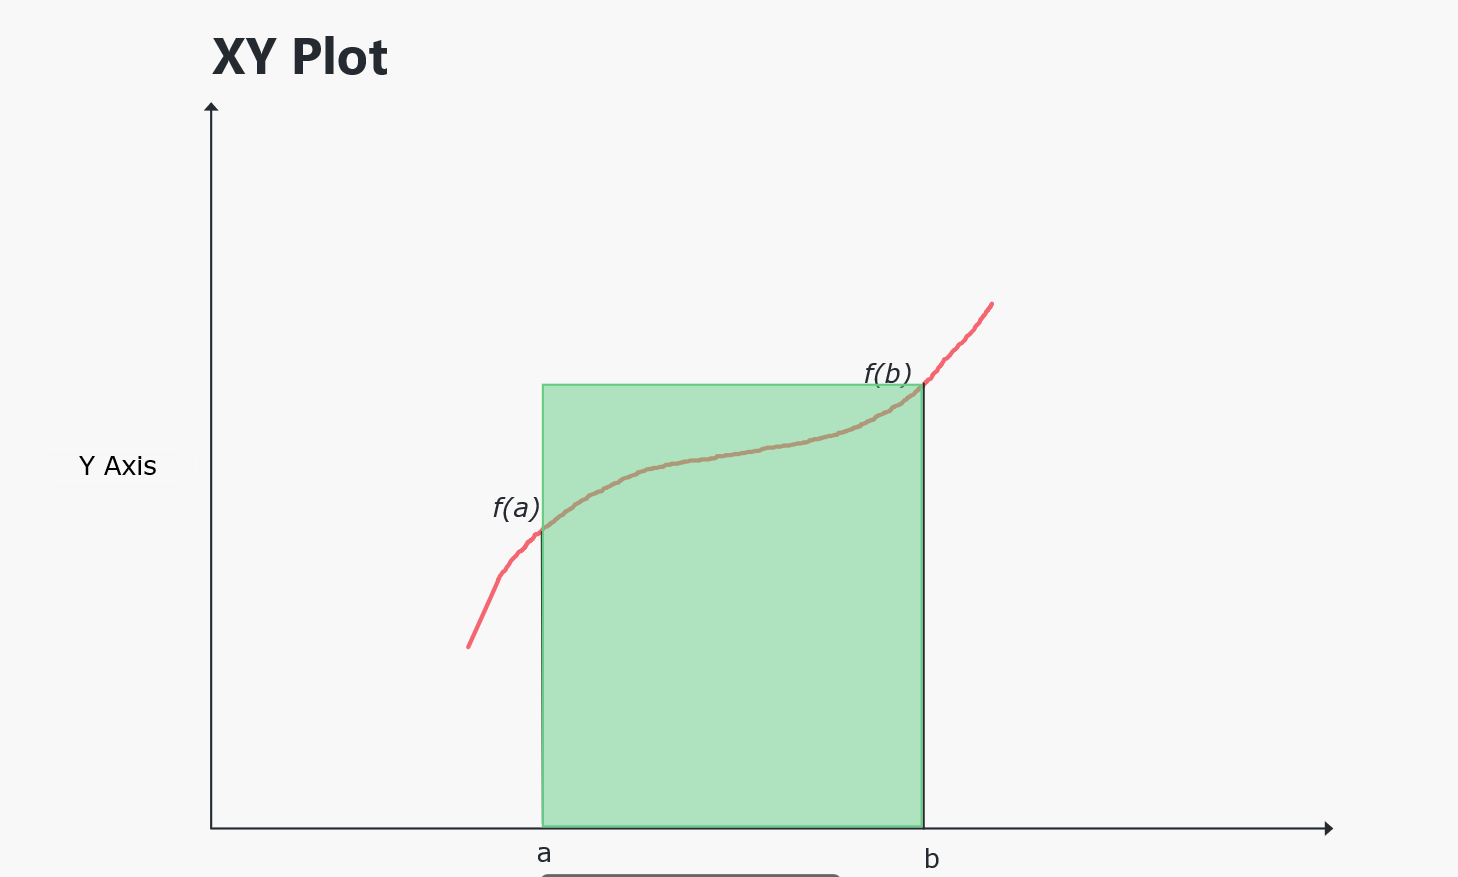
\includegraphics[scale=0.15]{Integrales3.png}}

\end{figure}
\noindent
De esta manera el cálculo del área bajo la curva que obtenemos es el siguiente
\begin{equation*}
\begin{array}{rr}
 inf(f(x))\cdot (b-a)& sup(f(x))\cdot(b-a)\\
\end{array}
\end{equation*}
\noindent
Es evidente que esto como aproximación del área bajo la curva deja bastante que desear, por tanto, se puede dividir el intervalo $[a,b]$ a la mitad de manera que se obtenga una mejor aproximación como se ve en la imagen.
\begin{figure}[H]
\centering
\graphicspath{{imagenes_analisis/}}
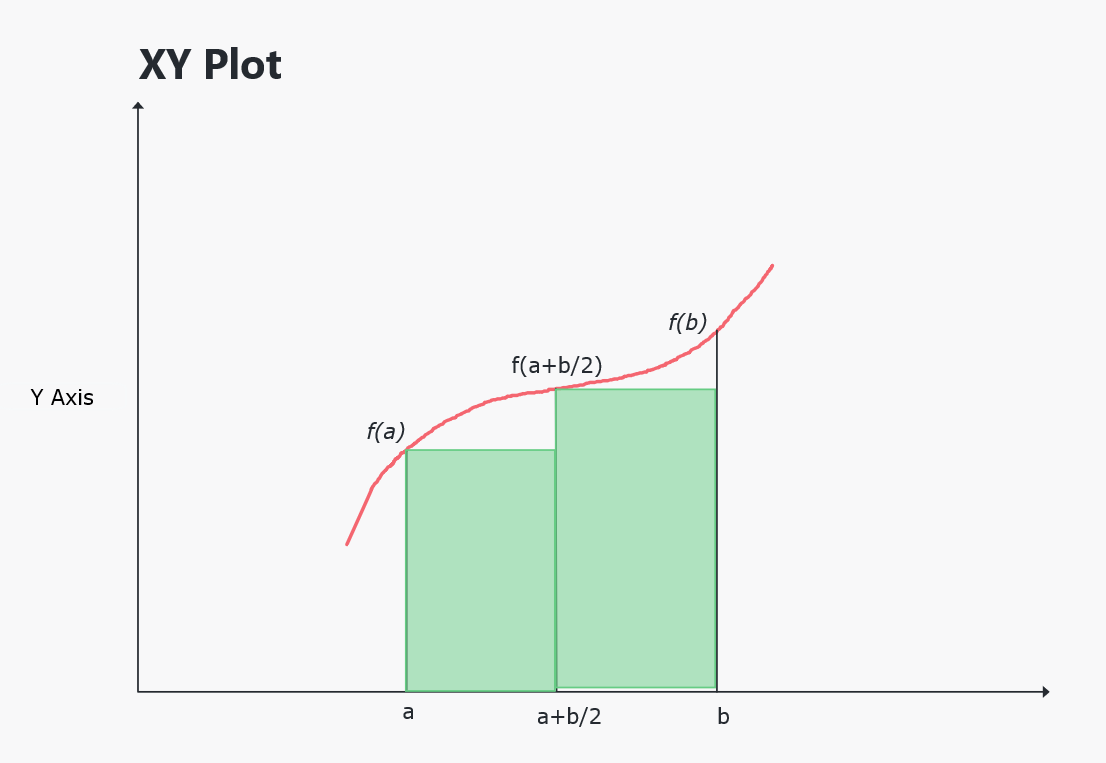
\includegraphics[scale=0.25]{Integrales4.png}
\label{Función $f(x)$}

\end{figure}
\noindent
Como se puede ver en este caso de las áreas por debajo, se aproxima de mejor manera el área por debajo.\\
\noindent 
En general, podemos hacer una partición de n partes del intervalo $[a,b]$, es decir, sean $\lbrace x_0,x_1\ldots x_n\rbrace$ donde $a=x_0<x_1\ldots<x_{n-1}<x_n=b$, de esta manera, tomar los rectángulos $r_i, R_i$ debajo o por encima de la curva respectivamente tomando como altura el mínimo o máximo de $f(x)$ en el intervalo $[x_{i-1},x_{i}]$ respectivamente.\\
\noindent
De esta manera, el área de cada rectángulo es $\displaystyle area(r_i)=\inf_{x\in{[x_{i-1},x_i]}}(f(x))\cdot (x_{i}-x_{i-1})$ , la suma de todos los rectángulos sería el área bajo la curva. 

Si hacemos una partición infinitesimal, es decir hacemos que el numero de los puntos $x_i$ lleguen a ser infinitos podemos obtener el área bajo la curva. 

\begin{defi}
Sea $f(x)$ una función real continua, una función es integrable si al hacer infinitas particiones, la suma superior (la suma de las áreas que toma los supremos) y la suma inferior (lo mismo pero con los mínimos). A ese limite se le llama \textit{\textbf{Integral de $f(x)$ en el intervalo $[a,b]$}}
\end{defi}
\newpage
\section{Cálculo efectivo de integrales}
\noindent
Muchas veces se considera el operador integral como el operador inverso de la derivada para calcular la integral tenemos que desarrollar varias técnicas 
\subsection*{Primitivas}
\begin{defi}
Sea una función $F(x)$ diremos que es \textbf{primitiva} de la función $f(x)\Leftrightarrow F'(x)=f(x)$
\end{defi}
\noindent
Para empezar, vamos a ver lo que se llaman \textbf{primitivas inmediatas}, es decir son las primitivas que no requieren ningún mecanismo más que las siguientes fórmulas

\subsection{Primitivas inmediatas}
Para empezar hay que tener en cuenta que las integrales son límites lo que implica que tenemos la siguiente propiedad.\\

Sean $f,g$ funciones integrables y $\lambda \in \mathbb{R}$ entonces tenemos que:
$$
\int f(x)+\lambda\cdot g(x )dx=\int f(x) dx+\lambda\int g(x) dx
$$
\noindent
Es decir la integral es un operador lineal sobre las funciones, ya que conserva las sumas de elementos y los productos de estos por escalares (Pero ya hablaremos de que es una aplicación lineal más tarde)

Aplicando esta propiedad y las fórmulas que se detallan a continuación podemos hacer bastantes integrales. A la izquierda se detalla como hacer la integral sobre nada más que una función y el derecho sobre una composición. \\
\begin{center}
\begin{tabular}{|c|c|}

\hline
$\displaystyle\int x^n =\dfrac{1}{n+1} x^{n+1}+C$ $\forall n\neq 1$&$\displaystyle\int f(x)^n \cdot f'(x)dx= \dfrac{1}{n+1}f(x)^{n+1}+C$  $\forall n\neq 1$\\[2ex]
\hline
$\displaystyle\int e^x dx=e^x+C$&$\displaystyle\int f(x)$\\
\hline
$\displaystyle\int \dfrac{1}{x}dx=ln|x|+C$&$\displaystyle\int \dfrac{f'(x)}{f(x)}dx=ln|f(x)|+C$\\
\hline
$\displaystyle\int cos(x)dx=sen(x)+C$&$\displaystyle\int f(x)$\\
\hline
$\displaystyle\int sen(x)dx=-cos(x)+C$&$\displaystyle\int f(x)$\\
\hline
$\displaystyle\int \dfrac{1}{\sqrt{1-x^2}}=arcsen(x)+C$&$\displaystyle\int f(x)$\\
\hline
$\displaystyle\int \dfrac{1}{1+x^2}=arctg(x)+C$&$\displaystyle\int f(x)$\\
\hline

\end{tabular}

\end{center}

\subsection{Integración por partes}
\subsection{Integración por cambio de variable}
\subsection{Integración de funciones racionales}
\subsection{Ejercicios}
\section{Aplicaciones de la integral}



